\iffalse METRICS
- Numerical stability of different conformal mapping methods
- Boundary discretization requirements (how smooth does $\gamma$ need to be?)
- Mesh quality preservation - how does the mapping affect triangle quality?
- Computational complexity
- Input and output formats
- https://www.desmos.com/calculator/g9asjc6xph
\fi
\section{Existing Methods}
This chapter aims to give an overview and compare some existing methods in terms of input/output format, requirements on the boundary or shape of the regions, computational complexity, numerical stability and mesh quality preservation/ accuracy. The list is non-exhaustive but covers some of the most well-known and widely used methods.

We start with an overview of the methods covered and how to choose between them depending on the application before explaining each of them in more detail.
%% THIS SHOULD GIVE A COMPREHENSIBLE OVERVIEW OF POTENTIAL METHODS AND HOW TO CHOOSE THEM
\begin{center}
    \red{maybe change to first boundary smooth then BIE, if not smooth then at least piecewise continuous then SCE, else if not well-behaved IDK}
\begin{tikzpicture}[node distance=1cm]

\node (BVP) {BVP};

\node (Q_poly) [below=of BVP] {$\Omega$ a polygon?};

\node (SCE) [right=of Q_poly] {Schwarz-Christoffel};

\node (Q_BIE) [below=of Q_poly] {Reformulate as BIE?};

\node (Q_star) [below=of Q_BIE] {$\Omega$ star-shaped?};

\node (theo) [below=of Q_star] {Theodorsen's Equation};

\node (BIE) [right=of Q_star] {General BIE Methods};
\node (kerz) [below=of BIE] {Kerzman-Stein};
\node (neu) [below left=of kerz, xshift=1cm] {Neumann Kernel};
\node (symm) [below right=of BIE] {Symm's Equation*};
\node (amano) [below=of symm] {Amano's Method};

\node (other) [right=of Q_BIE] {Other Method Families};
\node (zip) [above right=of other] {Zipper};
\node (berg) [right=of other] {Bergman Kernel};
\node (AP) [below right=of other] {Alternating Projections};

\draw [->] (BVP) -- (Q_poly);

\draw [->] (Q_poly) -- (SCE) 
    node [midway, above] {Yes};
\draw [->] (Q_poly) -- (Q_BIE) 
    node [midway, left] {No};

\draw [->] (Q_BIE) -- (Q_star) 
    node [midway, left] {Yes};
\draw [->] (Q_star) -- (theo) 
    node [midway, left] {Yes};
\draw [->] (Q_star) -- (BIE) 
    node [midway, above] {No};

\draw [->] (BIE) -- (kerz);
\draw [->] (BIE) -- (neu);
\draw [->] (BIE) -- (symm);
\draw [->] (BIE) -- (amano);

\draw [->] (Q_BIE) -- (other) 
    node [midway, above] {No};

\draw [->] (other) -- (zip);
\draw [->] (other) -- (berg);
\draw [->] (other) -- (AP);

\end{tikzpicture}
\end{center}

\begin{center}

\begin{tikzpicture}[
    node distance=0.6cm and 0.4cm, % Tight spacing
    every node/.style={font=\small, align=center},
    process/.style={draw=none, fill=none},
    decision/.style={draw=none, fill=none, font=\sffamily\bfseries\small},
    arrow/.style={->}
]

% --- The Central Spine (Aligned Vertically) ---
\node (start) [process] {BVP};
\node (dec_smooth) [decision, below=1cm of start] {$\partial \Omega$ Smooth ($C^1$)?};
\node (bie_group) [process, below=1cm of dec_smooth] {Boundary Integral\\Equations (BIE)};
\node (dec_star) [decision, below=1cm of bie_group] {$\Omega$ Star-shaped?};

% --- Star-Shaped Branches (Bottom of Spine) ---
% Left Branch: Theodorsen
\node (theodorsen) [process, left=1cm of dec_star] {Theodorsen's\\Method};

% Down Branch: General Smooth Methods
\node (general_bie_label) [process, below=1cm of dec_star] {General Smooth Methods:};
    % List
    \node (wegmann) [process, below=0.1cm of general_bie_label] {Wegmann's Method};
    \node (neumann) [process, below=0.1cm of wegmann] {Neumann Kernel};
    \node (amano) [process, below=0.1cm of neumann] {Symm's Eq. (Amano)};


% --- Polygon Branch (To the Right) ---
% Placed to the right of the first decision
\node (dec_poly) [decision, right=1.5cm of dec_smooth] {$\Omega$ a Polygon?};

    % Right Branch: Schwarz-Christoffel
    \node (schwarz) [process, right=1cm of dec_poly] {Schwarz-\\Christoffel};

    % Down Branch: General Jordan Curves
    \node (general_group) [process, below=1cm of dec_poly] {General Jordan\\Curves:};
    
    % List (Aligned with General Jordan Label)
    \node (zipper) [process, below=0.1cm of general_group] {Zipper Algorithm};
    \node (ap) [process, below=0.1cm of zipper] {Alternating\\Projections};
    \node (conjugate) [process, below=0.1cm of ap] {Conjugate Function};
    \node (prob) [process, below=0.1cm of conjugate] {Probabilistic\\Method};


% --- Arrows ---

% Spine flow
\draw [arrow] (start) -- (dec_smooth);
\draw [arrow] (dec_smooth) -- node[right, font=\scriptsize] {Yes} (bie_group);
\draw [arrow] (bie_group) -- (dec_star);

% Smooth -> Polygon (Straight Arrow request)
\draw [arrow] (dec_smooth) -- node[above, font=\scriptsize] {No} (dec_poly);

% Star-Shaped Decisions
\draw [arrow] (dec_star) -- node[above, font=\scriptsize] {Yes} (theodorsen);
\draw [arrow] (dec_star) -- node[right, font=\scriptsize] {No} (general_bie_label);

% Polygon Decisions
\draw [arrow] (dec_poly) -- node[above, font=\scriptsize] {Yes} (schwarz);
\draw [arrow] (dec_poly) -- node[right, font=\scriptsize] {No} (general_group);

% List Connectors (Optional thin lines for visual grouping)
\draw [thin, gray] (general_bie_label) -- (wegmann);
\draw [thin, gray] (wegmann) -- (neumann);
\draw [thin, gray] (neumann) -- (amano);

\draw [thin, gray] (general_group) -- (zipper);
\draw [thin, gray] (zipper) -- (ap);
\draw [thin, gray] (ap) -- (conjugate);
\draw [thin, gray] (conjugate) -- (prob);

\end{tikzpicture}

\end{center}

\subsection{Schwarz-Christoffel Method} \label{chap:SchwarzChristoffelMethod}
One class of methods for finding the conformal mapping $\psi$ is given by the Schwarz-Christoffel equation, which relates the derivative of $\psi$ to an integral over the boundary of the target domain $\Omega$ when $\Omega$ is a polygon.
\subsubsection{Preliminaries and Notation}
\begin{definition} [\cite{wiki:Polygon}]
    A \textbf{Polygon} is a piecewise linear Jordan curve with finitely many line segments connecting corner points $z_1, ..., z_N$.
\end{definition} 

For each $z_i\in\Gamma$, denote the exterior angle by $\measuredangle z_i=\theta_i\pi$. Then for any polygon we have $$\sum_{i=1}^{k} \theta_i = 2$$ and we set $\theta_i\in[-1,1]\forall i$. 
Note also that $P$ need not be bounded, since we can add vertices at complex infinity with exterior angles ranging from $[1,3]$. These angles are defined to be $2\pi$ minus the external angle formed in the plane by the two lines meeting at infinity \cite{Trefethen1980_SCnumericalcomputation}. 
\begin{center}
\begin{tikzpicture}[scale=.8]

    \begin{scope}[xshift=-8cm]%[shift=(-6,2)]
        \coordinate (Wk-2) at (0, 0);
        \coordinate (Wk-1) at (1.5, .5); % Intermediate point on the edge
        \coordinate (W_k) at (2.5, -0.5); % The corner vertex (labeled w_tilde_k)
        \coordinate (P_top_left) at (-0.5, 2.0);
        \coordinate (P_top_right) at (3.0, 1.3);
        \coordinate (W_k_angle) at (3.25, -1.25); % Position for angle arc
        \coordinate (W_k-2_angle) at (.25, -1); % Same as W_k for clarity

        \draw (P_top_left) -- (Wk-2) -- (Wk-1) -- (W_k) -- (P_top_right);
        
        \draw[dashed] (Wk-2) -- (W_k-2_angle); 
        \draw[dashed] (W_k) -- (W_k_angle); 

        \fill (Wk-2) circle (1.5pt) node[below left] {$z_{k-2}$};
        \fill (Wk-1) circle (1.5pt) node[above] {$z_{k-1}$}; % This is marked as an internal point on the edge
        \fill (W_k) circle (1.5pt) node[below left] {${z}_k$}; % This is the corner vertex
        \fill (P_top_right) circle (1.5pt); % Mark the point after w_tilde_k

        \node at (0.7, 1.5) {$P$};

        \pic [draw, -, angle radius=0.5cm, "$\theta_k$", angle eccentricity=1.7] 
            {angle = W_k_angle--W_k--P_top_right};
        \pic [draw, -, angle radius=0.5cm, "$\theta_{k-2}$", angle eccentricity=2]
            {angle = W_k-2_angle--Wk-2--Wk-1};
    \end{scope}

    \begin{scope}%[xshift=8]%[shift=(1,0)]
        \coordinate (z1) at (1, -1);
        \coordinate (z5) at (1, 1); 
        \coordinate (z3) at (-2, -1);
        \coordinate (z4) at (1, -1);
        \coordinate (z2) at (-.5,3);
        \coordinate (z0) at (3,-1); 
        \coordinate (z55) at (1, 2);

        \draw (z0) -- (z1) -- (z5) -- (z4) -- (z3) -- (z2);
        
        \fill (z1) circle (1.5pt) node[below] {$z_4=z_1$};
%        \fill (z2) circle (1.5pt) node[above] {$z_2$}; 
        \fill (z3) circle (1.5pt) node[below left] {$z_3$};
        \fill (z5) circle (1.5pt) node[right] {$z_5$};

        \node at (2, 1.5) {$Q$};
        \node at (z2) [right] {$z_2=\infty$\label{infty}};
        \node at (z2) [below right] {$\theta_2=\frac{4}{3}$};


        \pic [draw, -, angle radius=0.5cm, "$\theta_3$", angle eccentricity=1.7] 
            {angle = z4--z3--z2};
        \pic [draw, -, angle radius=0.5cm, "$\theta_1$", angle eccentricity=1.7]
            {angle = z0--z1--z5};
        \pic [draw, -, angle radius=0.3cm, "$\theta_5$", angle eccentricity=1.7]
            {angle = z55--z5--z4};
    \end{scope}

\end{tikzpicture}
\end{center}
\bigskip

\label{infinity}
In the above example $Q$ we have the two lines joining at $z_3$ again joining at infinity ($z_2$), where their outer angle is $\theta_2=2 - \theta_3 = \frac{5}{3}$, and thus the angles are 
$$\theta_1=\frac{1}{2}, \theta_2=\frac{5}{3}, \theta_3=\frac{1}{3}, \theta_4=\frac{1}{2}, \theta_5=-1 \implies \sum_{i=1}^{5} \theta_i = 2.$$
Now pick prevertices $v_1, ..., v_N \in \del\mathbb{D}$ as well as two constants $z_c,C\in\C$ (these choices will be explained later) and consider the Schwarz-Christoffel formula:
\begin{equation} % TREFETHEN W = MY Z, TREFETHEN Z = MY V
    z=\psi(v)= z_c + C\int_{0}^{v} \prod_{k=1}^{N} (1-\frac{\zeta}{v_k})^{-\theta_k} d\zeta
\end{equation}

Note that $1-\frac{\zeta}{v_k} \in \{|z-1|<1 \}$ for $|v|<1$. Hence we can define a branch of logarithm with branch cut along the negative real axis and define $(1-\frac{\zeta}{v_k})^{-\theta_k} = exp(-\theta_k \log(1-\frac{\zeta}{v_k}))$, $\psi(v)$ defines an analytic function on $\disk$ which is continuous except at the vertices $v_k$.
The formula is constructed such that the angles at the vertices correspong precisely to the exterior angles we need, hence the image of $\psi$ is a polygon with the correct angles. However, the lengths of the line segments need not be correct: This is where the choice of parameters $v_1, ..., v_N, z_c$ and $C$ comes in, and this is where the computational challenge in this method lies.
For the mapping to be unique, we can fix three of these parameters arbitrarily according to the Riemann mapping theorem. The remaining parameters are determined by solving the so-called \textbf{parameter problem}, which consists of a system of nonlinear equations obtained by enforcing the side lengths of the polygon to be correct.

For fixing of the initial three parameters one has two options in principle:
\begin{enumerate}
    \item Fix three of the prevertices $v_k$ on the unit circle.
    \item Fix only one prevertex and the point $z_c=\psi(0)\in P$. 
\end{enumerate}
The first option results in a remaining system of size $(N-3)\times(N-3)$ which is computationally more attractive, but may be too restrictive when scaling to polygons with many more vertices, as it can lead to very uneven distribution of the prevertices on the unit circle. Hence why the second option is often preferred, even though it means solving a $(N-1)\times(N-1)$ system \cite[page 84]{Trefethen1980_SCnumericalcomputation}.
Note that the Schwarz-Christoffel formula guarantees correctness of the angles and the prevertices are on the unit circle, hence defined by their angle; thus, it remains to tune lengths only, and our system of equations is actually real! 

Thus, the first step is to fix $v_N=1\in\disk$ (1 real degree of freedom) and $z_c\in P$ (two real degrees of freedom) the image of the origin under $\psi$. This yields uniqueness of the mapping.

Next, the scaling factor $C$ is defined by the formula 
\begin{equation} \label{eq:fix_v_N}
    \psi(v_N) - \psi(0) = z_N - z_C = C \int_{0}^{v_N=1} \prod_{k=1}^{N} (1-\frac{\zeta}{v_k})^{-\theta_k} d\zeta
\end{equation}
i.e. it is chosen such that the image of the segment from $v_N$ to the origin is correctly scaled to match the segment from $z_N$ to $z_c$.
Then a first vertex is pinned down to fix the "orientation" of the polygon (rotation anchoring):
\begin{equation} \label{eq:fix_v_1}
        z_1 - z_C = C \int_{0}^{v_1} \prod_{k=1}^{N} (1-\frac{\zeta}{v_k})^{-\theta_k} d\zeta
\end{equation}
This defines two real constraints, hence it remains to formulate $N-3$ equations for our $(N-1)\times (N-1)$ system.

\begin{center}
\begin{tikzpicture}[
    scale=.9,
    % Define styles for consistent drawing
    dot/.style={circle, fill=black, inner sep=1.2pt},
    target/.style={circle, draw=black, inner sep=2.5pt}, % Removed 'thick'
    axis/.style={densely dashed}, % Removed 'thick'
    maparrow/.style={->} % Removed 'thick' and 'Stealth' tip, now default
]

% ==========================================
% LEFT SIDE: The Unit Disk (v-plane)
% ==========================================
\begin{scope}[local bounding box=disk]
    % Radius
    \def\R{2}
    
    % Draw Circle (Standard line width)
    \draw (0,0) circle (\R);
    
    % Center 0
    \node[dot, label=above:$0$] (O) at (0,0) {};
    
    % Define coordinates for v points using polar angles
    \coordinate (v10) at (0:\R);
    \coordinate (v1)  at (40:\R);
    \coordinate (v2)  at (65:\R);
    \coordinate (v3)  at (105:\R);
    \coordinate (v4)  at (165:\R);
    \coordinate (v5)  at (200:\R);
    \coordinate (v6)  at (235:\R);
    \coordinate (v7)  at (275:\R);
    \coordinate (v8)  at (315:\R);
    \coordinate (v9)  at (340:\R);

    % Draw internal dashed lines (Radii)
    \draw[axis] (O) -- (v10);
    \draw[axis] (O) -- (v1);
    \draw[axis] (O) -- (v5);
    \draw[axis] (O) -- (v7);
    \draw[axis] (O) -- (v9); 
    
    % Draw internal dashed chords
    \draw[axis] (v3) -- (v4);
    \draw[axis] (v4) -- (v5);
    \draw[axis] (v9) -- (v10);

    % Draw Dots
    \foreach \n in {1,2,3,4,5,6,7,8,9} {
        \node[dot] at (v\n) {};
    }
    % v10 is a target circle
    \node[dot] at (v10) {};
    \node[target] at (v10) {};

    % Labels
    \node[right] at (v10) {$v_{10}$};
    \node[right] at (v1) {$v_1$};
    \node[above] at (v2) {$v_2$};
    \node[above] at (v3) {$v_3$};
    \node[left] at (v4) {$v_4$};
    \node[left] at (v5) {$v_5$};
    \node[below] at (v6) {$v_6$};
    \node[below] at (v7) {$v_7$};
    \node[right] at (v8) {$v_8$};
    \node[right] at (v9) {$v_9$};

\end{scope}

% ==========================================
% ARROW: The Mapping psi
% ==========================================
% Changed label to psi, used default arrow style
\draw[maparrow] ($(disk.east)+(0.5,0)$) -- node[above, font=\large] {$\psi$} ($(disk.east)+(2.5,0)$);


% ==========================================
% RIGHT SIDE: The Polygon (z-plane)
% ==========================================
\begin{scope}[xshift=8cm, yshift=0cm]
    
    % Center z_c
    \coordinate (zc) at (-0.5,0);
    \node[dot, label=left:$z_c$] at (zc) {};

    % Define Vertices
    % Right Wall
    \coordinate (z10) at (1.5, 0.5);
    \coordinate (z1)  at (2.2, 2.0);
    \coordinate (z9)  at (2.2, -1.0);
    
    % Left Wall Structure
    \coordinate (z3)  at (0.0, 2.0);
    \coordinate (z4)  at (-0.8, 0.5);
    \coordinate (z5)  at (-1.8, -0.8);
    \coordinate (z7)  at (-0.2, -1.8);

    % --- DRAW BOUNDARIES (Standard line width) ---
    
    % Right Wall (Infinite up/down)
    \draw (z1) -- (z10) -- (z9);
    \draw (z1) -- +(0, 0.5);   % Up to infinity
    \draw (z9) -- +(0, -1.8);  % Down to infinity

    % Left Wall Top (Infinite up)
    \draw (z3) -- +(0, .5);
    
    % Left Wall Middle Bump
    \draw (z3) -- (z4) -- (z5);
    
    % Left Wall Exit
    \draw (z5) -- +(-2.5, 0);  % Left to infinity

    % Bottom Wall Feature (z7)
    \draw (z7) -- +(-3.0, -1.0); % Angled down-left
    \draw (z7) -- +(0, -1);    % Straight down

    % --- DRAW MAPPED LINES (Dashed Curves) ---
    
    % zc to z10
    \draw[axis] (zc) .. controls (0.5, 0.7) .. (z10);
    
    % zc to z1
    \draw[axis] (zc) .. controls (0.5, 1.5) .. (z1);
    
    % zc to z9
    \draw[axis] (zc) .. controls (0.3, -0.9) .. (z9);
    
    % zc to z7
    \draw[axis] (zc) .. controls (-0.3, -1.0) .. (z7);
    
    % zc to z5 (S-curve)
    \draw[axis] (zc) .. controls (-0.8, -0.2) and (-1.0, -0.5) .. (z5);

    % Chord z3 to z4
    \draw[axis] (z3) .. controls (-0.2, 1.0) .. (z4);
    
    % Chord z9 to z10
    \draw[axis] (z9) .. controls (1.8, -0.2) .. (z10);
    
    % Chord z1 to z10
    \draw[axis] (z1) .. controls (1.5, 1.5) .. (z10);

    % --- DOTS AND LABELS ---

    \foreach \pt/\pos in {z1/right, z3/left, z4/left, z5/above left, z7/below left, z9/right} {
        \node[dot] at (\pt) {};
    }
    \node[right] at (z1) {$z_1$};
    \node[right] at (z9) {$z_9$};
    \node[right] at (z7) {$z_7$};
    \node[above left] at (z5) {$z_5$};
    \node[left] at (z4) {$z_4$};
    \node[left] at (z3) {$z_3$};
    
    % z10 Target
    \node[dot] at (z10) {};
    \node[target] at (z10) {};
    \node[right] at (z10) {$z_{10}$};

\end{scope}

\end{tikzpicture}
\end{center}

These are found by enforcing the side lengths of the polygon to be correct between the remaining vertices.
\begin{equation} \label{eq:N-3sidelengths}
        |z_{i+1} - z_i| = |C \int_{v_i}^{v_{i+1}} \prod_{k=1}^{N} (1-\frac{\zeta}{v_k})^{-\theta_k} d\zeta| \quad  \forall i\in 2, ..., N-2
\end{equation}
Note that unboundedness of the polygon is not a problem, since it can be modeled by one vertex as described earlier (\ref{infinity}), which can be chosen to be $z_N$ without loss of generality; this way, it will be taken care of by the first equation (\ref{eq:fix_v_N}) and will not pose a problem when comparing lengths in (\ref{eq:N-3sidelengths}).

\iffalse
The system of equations then consists of the 2N conditions
\begin{equation}
    z_{k}-z_c = C\int_{0}^{v_{k}} \prod_{i=1}^{N} (1-\frac{\zeta}{v_i})^{-\theta_i} d\zeta \quad \text{ for } k=1,...,N.
\end{equation}
Note this system is highly overdetermined, so the tricky problem to solve is to delete $2N+1$ of those conditions without leaving any degrees of freedom in the final system. 


These arcs being smooth yields tangents with well-defined derivatives at every point of the boundary curves except for (a finite number of) corners, and we denote the angles of these tangents with $\theta_{\mathbb{D}}(s_{\mathbb{D}})$ and $\theta_{\Omega}(s_{\Omega})$ respectively. If $z_0$ is a corner it will have a turning angle of 
$$\measuredangle\theta_{\mathbb{D}}(z_0)=\theta_{\mathbb{D}}(z_0+\eps)-\theta_{\mathbb{D}}(z_0-\eps),$$ 
where $\eps\to0$ \red{is this eps in 0,2pi or is it on the boundary, and if theta(s) for s in 0,2pi and z0 on boundary how can the above equation be well-def even}. The same applies to corners of $\Omega$. Then,
$\frac{\del\theta_{\mathbb{D}}}{\del s_{\mathbb{D}}} = \measuredangle\theta_{\mathbb{D}}(z_0)\delta(s_{\mathbb{D}}-z_0)$ for $\delta$ the Dirac function, and similarly for $\theta_{\Omega}$ and thus $\theta_{\mathbb{D}}$ and $\theta_{\Omega}$ are piecewise continuously differentiable functions with jump discontinuities at the corner points.

%\red{\subsubsection{the log derivative of Phi}}

\subsubsection{Green's Functions}
A Green's function is a general concept for solving differential equations containing a linear operator.
\begin{definition} 
    A \textbf{Green's function} or \textbf{Green function $G(x,s)$} is any solution to $$LG(x,s)=\delta(x-s)$$ where $L=L(x)$ is a linear operator acting on distributions over $\R^{n}$ and $\delta$ is the Dirac delta function.
\end{definition}
This definition can be exploited to solve inhomogeneous differential equations of the form $Lu=f(x)$.
In the case of the SCE the Green's function are defined as $G(z,z'):\mathbb{D}\to\mathbb{R}$ satisfying $$\nabla^2 G(z,z') = 2\pi \delta(u-u')\delta(v-v') $$ inside the disk and $$\frac{\del G(z_B, z')}{\del n} = \beta_i$$ where $n$ is the outward normal vector at the boundary point $z_B \in \del\mathbb{D}$ and $\beta_i$ is a real constant associated with the $i$'th arc's length $l_i$ such that $\sum l_i\beta_i = 2\pi$. It can be shown according to Floryan and Zemach that this defines a unique Green's function up to an additive constant \cite{FLORYAN1987_SC_general}.
The SCE can be written explicitly whenever the Green's function is \red{obtainable in closed analytic form, i.e. expressable via a finite number of elementary operations (is that what is meant on p348? i looked up wikipedia for closed analytic form)}.

\subsubsection{Schwarz-Christoffel Equation Variants}
Let $\mathcal{G}(z, z_B')$ be a complex extension of the above defined $G(z,z_B')$, i.e. $\mathcal{G}(z, z_B')$ is analytic with real part $G(z,z_B')$.
A Schwarz-Christoffel equation for a conformal mapping $\Phi(z):\mathbb{D}\to\Omega$ has the form $$ log \frac{d\Phi}{dz}= C+\displaystyle\sum_i Q_i,$$ where $C\in\mathbb{C}$ is a constant and the $Q_i$ are the Green's function integrals over the boundary arcs of $\mathbb{D}$.
Some parameters and constants have to be determined in order to get a unique $\Phi$ for a particular given $\Omega$. The Riemann mapping theorem allows \red{HOW?} for the first three real parameters to be preassigned, for example to three boundary points in the case of simply connected bounded $\Omega$. The remaining degrees of freedom must be solved for using properties of the arcs $s_{\Omega}(s_z)$ and $s_{\mathbb{D}}(s_z)$. 

The most general form is called Schwarz-Christoffel equation with subtraction \cite{FLORYAN1987_SC_general}:
$$log(\frac{d\Phi}{dz}) = C_0 - \frac{1}{2\pi}\displaystyle\int_{\del\mathbb {D}} [\mathcal{G}(z, z_B')-\mathcal{G}(z_0, z_B')] \times [d\theta_{\Omega}(s_z')-d\theta_{\del\mathbb{D}}(s_z')]$$
where $C_0\in\mathbb{C}$ is a constant, $z_0$ is a fixed point in $\mathbb{D}$\red{or del?}, $\mathcal{G}(z,z_B')$ is the fundamental solution of the Laplace equation in $\del\mathbb{D}$ with singularity at $z_B' \in \del\mathbb{D}$\red{not at the boundary of omega?}. However, we can use an unsubtracted form of this equation since the integrals converge separately and we know our $\Omega$ is bounded (hence we need not care about behaviours at infinity), yielding the simpler form
$$log(\frac{d\Phi}{dz}) = C - \frac{1}{2\pi}\int_{\del\mathbb{D}} \mathcal{G}(z, z_B') [d\theta_{\Omega}(s_z')-d\theta_{\del\mathbb{D}}(s_z')]$$


\subsubsection{Implementation}
\cite{Brown1990_SC_meshgen}
\cite{Trefethen1980_SCnumericalcomputation}
\cite{banjaitrefethen2006_SCmultipolemethod}
\cite{Bezrodnykh2022_lauricella}
Crowding is a problem because it yields exponential derivative of $\Phi$, but can be fixed. \cite{Banjai2008_SC_crowdingworkaround}
\fi


\subsection{Zipper Method}\label{chap:ZipperMethod}
This algorithm was found independently by Kühnau and Marshall in the 1980's and has the advantage of finding $\psi$ and its inverse at the same time. 
The computed map is only approximately conformal, and is obtained as a composition of conformal maps onto slit halfplanes. Depending on the shape of the slits, the Zipper algorithm looks a bit different. 
In this section we will focus on the easiest version called the "geodesic algorithm" \cite{marshall2006_convergencezipperalgorithmconformal}.
First, let us introduce the following definition:

\subsubsection{Möbius Transforms}
\begin{definition}[{\cite{wiki:MoebiusTransform}, \cite[page 209]{SteinShakarchi2003_complexanalysis}}]
    A \textbf{Möbius transform} is a function on the extended complex plane $\hat\C:=\C\cup\{\infty\}$ which is uniquely determined by where it sends three points. It has the form
    $$ f(z) = \frac{az + b}{cz + d} $$
    with complex numbers $a,b,c,d$ such that $ad - bc \neq 0$.
\end{definition}
More explicitly, given three distinct points $z_1,z_2,z_3 \in \C$ and three distinct points $w_1,w_2,w_3 \in \C$ there exists a unique Möbius transform $f$ such that $f(z_i) = w_i$ for $i=1,2,3$:
$$ f(z)=\frac{(z-z_1)(z_2-z_3)}{(z-z_3)(z_2-z_1)}$$
In particular, Möbius transforms are conformal and more general than affine maps, since they can e.g. map $\infty$ to $0$ and vice versa.

\subsubsection{The Geodesic Algorithm}
The most elementary version of this algorithm is based on a function 
$$f_a: \mathbb{H}\setminus \gamma \to \mathbb{H}$$
where $\mathbb{H}$ is the upper half plane and $\gamma$ is a circular arc from $0$ to $a\in\mathbb{H}$ which is orthogonal to the real axis. The orthogonal circle also meets the real axis again at $b=|a^2|\text{Im}(a)$. Then the map can be expressed in closed form as 
$$f_a(z) = \sqrt{g_a \circ h_a (z)}$$ where $g_a(z) = z^2 + c^2$, $c=\frac{|a^2|}{\text{Im}(a)}$ is called the \textbf{conformal capacity} of $\gamma$ and $h_a(z) = \frac{z}{1-z/b}$.

%\documentclass[tikz,border=10pt]{standalone}
%\usetikzlibrary{calc,positioning}
%\usepackage{amsfonts}
%\begin{document}

\bigskip

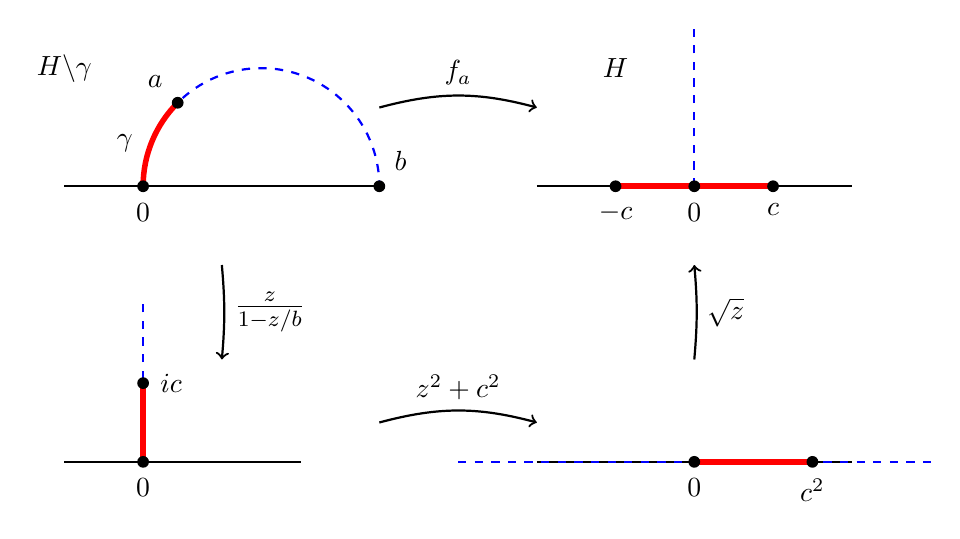
\begin{tikzpicture}[thick,
  dot/.style={fill=black,circle,inner sep=1.5pt}]

% Top left: H \ gamma
\begin{scope}[shift={(-4,2)}]
  \draw (-1,0) -- (3,0);
  \draw[dashed,blue] (0,0) arc[start angle=180,end angle=0,radius=1.5];
  \draw[red,line width=2pt] (0,0) arc[start angle=180,end angle=135,radius=1.5];
  \node[dot,label=below:$0$] at (0,0) {};
  \node[dot,label=above left:$a$] at ({-1.5*cos(45)+1.5},{1.5*sin(45)}) {};
  \node[dot,label=above right:$b$] at (3,0) {};
  \node[above left] at (0,0.3) {$\gamma$};
  \node at (-1,1.5) {$\mathbb{H}\backslash\gamma$};
\end{scope}

% Arrow from top left to top right
\draw[->] (-1,3) to[bend left=15] node[above] {$f_a$} (1,3);

% Top right: H
\begin{scope}[shift={(3,2)}]
  \draw (-2,0) -- (2,0);
  \draw[dashed,blue] (0,0) -- (0,2);
  \draw[red,line width=2pt] (-1,0) -- (1,0);
  \node[dot,label=below:$-c$] at (-1,0) {};
  \node[dot,label=below:$0$] at (0,0) {};
  \node[dot,label=below:$c$] at (1,0) {};
  \node at (-1,1.5) {$\mathbb{H}$};
\end{scope}

% Arrow from top left to bottom left
\draw[->] (-3,1) to[bend left=5] node[right, font=\large] {$\frac{z}{1-z/b}$} (-3,-0.2);

% Arrow from top right to bottom right
\draw[<-] (3,1) to[bend left=5] node[right] {$\sqrt{z}$} (3,-0.2);

% Bottom left
\begin{scope}[shift={(-4,-1.5)}]
  \draw (-1,0) -- (2,0);
  \draw[dashed,blue] (0,0) -- (0,2);
  \draw[red,line width=2pt] (0,0) -- (0,1);
  \node[dot,label=below:$0$] at (0,0) {};
  \node[dot,label=right:$ic$]at (0,1) {};
% \node[blue,right] at (0,0.5) {$ic$};
\end{scope}

% Arrow from bottom left to bottom right
\draw[->] (-1,-1) to[bend left=15] node[above] {$z^2+c^2$} (1,-1);

% Bottom right
\begin{scope}[shift={(3,-1.5)}]
  \draw (-2,0) -- (2,0);
  \draw[dashed,blue] (-3,0) -- (3,0);
  \draw[red,line width=2pt] (0,0) -- (1.5,0);
  \node[dot,label=below:$0$] at (0,0) {};
  \node[dot,label=below:$c^2$] at (1.5,0) {};
\end{scope}
\end{tikzpicture}

\bigskip

%\end{document}

Now suppose $z_0, z_1, ..., z_n$ are points arranged counterclockwise on a Jordan curve $\Gamma$ in the upper half plane. The geodesic algorithm basically iterates over the arcs from $z_i$ to $z_{i+1}$ and "unzips" them one by one using the map $f_{a_i}$ where $a_i$ is the image of $z_{i+1}$ under the composition of all previous maps.
The original geodesic algorithm proposed by Marshall and Rohde constructs a conformal map from the upper half plane to the region bounded by $\Gamma$, but it can be adapted to map from the unit disk as well via a Möbius transformation mapping the half plane to the unit disk and back first.

\begin{algorithm}
    \caption{Geodesic Zipper Algorithm}
    \begin{algorithmic}
    \STATE \textbf{Input:} Points $z_0, z_1, ..., z_n$ on a Jordan curve $\Gamma$ in the upper half plane.
    \STATE \textbf{Output:} $\psi$: conformal map from $\mathbb{H}$ to the region bounded by $\Gamma$ and its inverse $\psi^{-1}$.
    \STATE $\varphi_1(z) := i\sqrt{(z-z_1)/(z-z_0)}$
    \STATE $\zeta_2:= \varphi_1(z_2)$
    \STATE $\varphi_2(z) := f_{\zeta_2}(z)$
    \FOR{k in n}
        \STATE $\zeta_k := \varphi_{k-1} \circ \ldots \circ \varphi_1 (z_k)$
        \STATE $\varphi_k(z) := f_{\zeta_k}(z)$
    \ENDFOR
    \STATE Finally, $\zeta_{n+1} := \varphi_n \circ \ldots \circ \varphi_1 (z_{0})\in\R$ and $\varphi_{n+1}(z) := -(\frac{z}{1 - z/\zeta_{n+1}})^2$
    \STATE Then $\psi(z) := \varphi_1^{-1} \circ \varphi_2^{-1} \circ \ldots \circ \varphi_{n+1}^{-1}(z)$ and $\psi^{-1}(z) := \varphi_{n+1} \circ \ldots \circ \varphi_2 \circ \varphi_1 (z)$
    \end{algorithmic}
\end{algorithm}
\begin{flushleft}
\includegraphics[width=\textwidth]{zipper_geodesic.png}
\end{flushleft}

\subsubsection{The Slit Algorithm}
The above geodesic algorithm is only as accurate as the approximation of the boundary curve $\Gamma$ by circular arcs between the points $z_i$. A more accurate version is given by the slit algorithm, which uses straight line segments instead of circular arcs.
We therefore exchange the map $f_a$ for a map $g_a: \mathbb{H}\setminus L \to \mathbb{H}$ where $L$ is the line segment from $0$ to $a\in\mathbb{H}$. This map does not have a closed form expression, but can be computed numerically using Newton's method.

\subsubsection{The Zipper Algorithm}
The approximation of $\Gamma$ by circular arcs or straight line segments can be further improved by using circular arcs which meet $\Gamma$ tangentially at the points $z_i$. Each arc is determined by the points $z_i, z_{i+1}$ and $z_{i+2}$, hence we assume an even number of boundary points. 
The first arc is replaced by $$\varphi_1(z)=\sqrt{\frac{(z-z_2)(z_1-z_2)}{(z-z_0)(z_1-z_2)}}.$$ At each subsequent step that circular arc through $\zeta_k$ and $\zeta_{k+1}$ is mapped onto a straight line segment by a Möbius transform, and then the Slit Algorithm is applied to unzip that segment.
This yields a sort of "quadratic approximation" of $\del\Omega$ instead of a linear one \cite[page 8]{marshall2006_convergencezipperalgorithmconformal}.

% \subsection{Shirokova's Method}
% \cite{Shirokova2014}

\subsection{Conjugate Function Method } \label{chap:ConjugateFunctionMethod}
Hakula, Quach and Rasila \cite{Hakula_2013_conjugatefunctionmethod} presented a new method in 2010 which is based on solving the Laplace equation subject to Dirichlet-Neumann mixed-type boundary conditions by exploiting geometric properties of quadrilaterals.  
\begin{definition}[{\cite[Definition 2.1]{Hakula_2013_conjugatefunctionmethod}}]
    A Jordan domain $\Omega\in\C$ with marked (positively ordered) points $z_1 , z_2 , z_3 , z_4 \in \del\Omega$ is called a \textbf{quadrilateral}, and is denoted by $$Q = (\Omega; z_1 , z_2 , z_3 , z_4 ).$$ 
    Then there is a canonical conformal map of the quadrilateral $Q$ onto a rectangle $$R_h = (\Omega ' ; 1 + ih, ih, 0, 1)$$ with the vertices corresponding, where $h$ defines the unique \textbf{modulus} of a quadrilateral $Q$. 
    We write $$M(Q) = h.$$
    Note that the reciprocal identity holds:
    \begin{equation}
        M(Q)M(\tilde{Q}) = 1
    \end{equation} 
    where $\tilde{Q} = (\Omega; z_2 , z_3 , z_4 , z_1 )$ is the \textbf{conjugate quadrilateral} of $Q$.
\end{definition}
The method solves a PDE directly on the mesh on the entire domain $\disk$ instead of only on the boundary in order to get the real part $u$ of $\psi=u+iv$. The special feature then is that the conjugate function $v$ is constructed by remarking that $v$ solves the same PDE as $u$ but with swapped boundary conditions. 
This second PDE is called the \textbf{dual problem}.
Thus, the method essentially consists of solving two symmetric Laplace problems on the entire domain with different boundary conditions and combining their solutions to get $\psi$.
The authors claim accuracy comparable with that of the standard Schwarz-Christoffel toolbox for both convex and non-convex quadrilaterals \cite[Figure 5]{Hakula_2013_conjugatefunctionmethod}.

\subsection{Probabilistic Uniformization Method} \label{chap:ProbabilisticMethod}
In 2007, Binder, Braverman ans Yampolsky \cite{binder2007_computationalcomplexityriemannmapping} proposed a method for finding a conformal map using a random walks solver to the general Dirichlet problem. They conjectured an upper bound of polynomial space and time for an algorithm with precision $\frac{1}{n}$ pixels (for explicitly given $\del\Omega$; quadratic if $\del\Omega$ is given only approximately, via a so-called \textit{oracle}, sort of a Dirac delta function). 
This method poses no constraints on the target region, but accuracy is unpredictable by definition.

\subsection{Theodorsen's Method} \label{chap:TheodorsenMethod}
For $\Omega$ star-shaped with regard to the origin, Theodorsen's method \cite[page 64]{Gaier1964} can be used to find the conformal mapping $\psi:\disk\to\Omega$ satisfying the initial conditions (\ref{eq:InitialConditionsOnPsi}).
Since $\Omega$ is star-shaped, the boundary $\Gamma$ can be parametrized by the polar angle. Consequently, the boundary correspondence function $S(\varphi)$ defined in (\ref{eq:boundaryCorrespondence}) becomes the angular function $\theta(\varphi)$. 
Theodorsen's integral equation is derived as follows:
Note points on the unit circle are parametrised by $e^{i\varphi}$ while $\Gamma$ can be parametrised by $\rho(\theta)e^{i\theta}$ for $\varphi, \theta\in[0,2\pi]$ and $\rho(\theta)>0$ the radius function of $\Gamma$ (by star-shapedness of $\Omega$). Thus, the problem reduces to relating $\varphi$ and $\theta$ via a function $\theta(\phi)$.
The trick is to introduce an auxiliary function involving a $\log$, which allows to separate the real and imaginary part of the problem: 
\begin{equation}
    Re^{i\alpha} = \log(R) + i\alpha
\end{equation} 
However, $\log$ has a singularity at $0$ which impedes direct application of the $\log$ as it contradicts with our normalization criterion on $\psi$ (\ref{eq:InitialConditionsOnPsi}).
Thus the singularity is removed by dividing out $z$. This gives us the helper function 
\begin{equation}\label{eq:helperfunctiontheodorsen}
    F(z) := \log(\frac{\psi(z)}{z}) = \\ 
    \log(\frac{\rho(\theta)e^{i\theta}}{e^{i\varphi}}) = \log(\rho(\theta)e^{i(\theta-\varphi)}) = \log(\rho(\theta))+i(\theta - \varphi).
\end{equation}
By the section on conjugate functions \ref{eq:operatorK} the real and imaginary parts of this helper function are conjugate. Thus, we can relate them by
\begin{equation}
    \theta - \varphi = K \log(\rho(\theta))
\end{equation}
which can be rewritten into Theodorsen's integral equation
\begin{equation}
    \theta(\varphi) = \varphi + K \log(\rho(\theta(\varphi))).
\end{equation}

The discretization as in \cite{Gutknecht1983_theodorsen_equation_FFT} is done by naming the difference between the boundary angle and the circle angle $Y := \theta - \varphi = \theta(\varphi) - \varphi$ the conjugate function of $X:= \log(\rho(\theta))= \log(|\eta(\varphi)|)$.
Theodorsen's integral equation becomes the fixed point equation
\begin{equation}\label{eq:TheodorsenDiscretized}
    y=\psi(y):=K_{\Sigma} \log(|\eta(\varphi+y)|)
\end{equation} 
where the equation is evaluated on a grid of $2N$ equidistant angles $\varphi_k = \frac{k\pi}{N}$ for $k=0, \dots, 2N-1$. Here, the vector $y$ approximates the values of the continuous function $Y(\varphi)$ at these grid points, such that $y_k \approx Y(\varphi_k)$.
The product $y$ can be computed efficiently using FFT (see chapter \ref{operatorK_N}).
\iffalse
If the discretization is based on trigonometric interpolation, $K_{\Sigma}$ is called \textbf{Wittich's matrix} \cite{Gutknecht1983_theodorsen_equation_FFT}.
By a permutation $P$ the above components can be brought to the form
\begin{equation}
    PK_{\Sigma}P =
    \begin{pmatrix}
        0 & -L^T \\
        L & 0
    \end{pmatrix}, \quad
    Py = \begin{pmatrix}
        y^{"} \\
        y^{' }
    \end{pmatrix}, \quad
    Ps = \begin{pmatrix}
        s^{"} \\
        s^{'}
    \end{pmatrix}.
\end{equation}
By Niethammer, (\ref{eq:TheodorsenDiscretized}) can be solved using nonlinear successive over-relaxation (SOR) for given $y_0^{"}, y_0^{'}$ and $\omega$ (relaxation factor) and $m\geq 0$:
\begin{equation}\label{eq:SOR}
    \begin{matrix}
        y_{m+1}^{"} &:= &(1-\omega)&y_m^{"} &- &\omega L^T \log(\eta(s^{'} + y_m^{'})) \\
        y_{m+1}^{'} &:= &(1-\omega)&y_m^{'} &+ &\omega L \log(\eta(s^{"} + y_m^{"}))        
    \end{matrix}
\end{equation}
Alternatively, nonlinear Jacobi iteration with relaxation (JOR) can be used:
\begin{equation}\label{eq:JOR}
    \begin{matrix}
        y_{m+1} &:= &(1-\omega)&y_m + &\omega \psi(y_m).
    \end{matrix}
\end{equation}
\fi
In case of $\Gamma$ not being smooth, Theodorsen's method becomes inaccurate \cite{Gutknecht1983_theodorsen_equation_FFT}.
It also theoretically needs $\Omega$ to be star-shaped in order to converge \cite{Wegmann1978_newtonverfahren}, since otherwise the radius function $\rho(\theta)$ becomes multivalued causing numerical failure, but has the advantage of being an easily computable fixed point equation if star-shaped. 
In practice, the star-shape requirement can also be relaxed by smoothing the boundary curve first using preliminary maps \cite{Gutknecht1983_theodorsen_equation_FFT}.


\subsection{Amano's Method of Fundamental Solutions} \label{chap:AmanosMethod}
A potential theoretic formulation of the conformal mapping problem leads to a Fredholm integral equation of the first kind, known as Symm's integral equation, which has a kernel with logarithmic singularity. 
Unlike Fredholm integral equations of the second kind like Theodorsen's equation, where the singularity of the kernel creates numerical instabilities, Symm's equation is easily solvable by numerical methods \cite[Chapter 9.1]{Kythe1998_symmsintegralequation}. One of these is Amano's method.
Conceptually, a pair of conjugate harmonic functions are expressed by a complex logarithmic potential, and the mapping problems are reduced to singular Fredholm integral equations of the first kind. Gaier \cite{Gaier1964} mathematically studied Symm’s integral equation and proved the existence and uniqueness of the solution. These methods need $\bigO(N^3)$ operations if the boundary is discretized at N points. Henrici showed that complexity of $\bigO(N^2\log N)$ can be achieved by using FFTs \cite{Henrici1986_vol3}.

\begin{definition}[{\cite[§ 4]{Amano1998_Amanosmethod}}]
    In two dimensions, the Laplace equation has a fundamental solution of the form $\log(r)$ where $r=|z-\zeta_k|$ is the modulus of the vector from any point $z$ on the region to the boundary point $\zeta_k$, $k\in N$. This function $\log(|z-\zeta_k|)$ is called the \textbf{logarithmic potential}. 
\end{definition}
A potential theoretic formulation of the Dirichlet problem (\ref{eq:DirichletProblem}) leads to a Fredholm integral equation of the first kind called \textbf{Symm's equation}
\begin{equation}\label{eq:Symm}
    \int_{\Gamma} \log| z - \zeta| \mu(\zeta) d\zeta = -\log|z| \quad \text{ for } z\in\Omega, \zeta\in\Gamma
\end{equation} which has a kernel with logarithmic singularity. In this context, the conformal mapping problem reduces to finding a suitable source density function $\mu(z)=g(z)+ih(z)$ on the boundary $\Gamma$ where $g$ and $h$ are conjugate and $g$ satisfies 
\begin{equation}
    \begin{matrix}
        \nabla^2 g(z) = 0 & z\in \Omega \\
        g(z) = -\frac{1}{2} \log|z\bar{z}| & z\in \Gamma.
    \end{matrix}
\end{equation}
It is more easily solvable by numerical methods than Fredholm integral equations of the second kind, where the kernel might have singularities near the boundary \cite[Chapter 9]{Kythe1998_symmsintegralequation}.

This is used in the so-called Charge Simulation Method which Amano's Method is based on.

\subsubsection{Algorithm}
The charge simulation method approximates the solution of the Laplace equation by a linear combination of fundamental solutions placed at so-called charge points outside the domain \cite{Amano1998_Amanosmethod} by 
\begin{equation}\label{eq:AmanosApproximation}
    g(z) = \sum_{k=1}^{N} Q_k log(|z-\zeta_k|),
\end{equation}
where $\zeta_1, \ldots, \zeta_N \notin\overline\Omega$ are called \textbf{charge points} and placed outside the domain. The unknown constants $Q_1, \ldots, Q_N$ are called \textbf{charges} and determined to satisfy the boundary condition at the \textbf{collocation points} $z_1, \ldots, z_N$ (fixed check points on the boundary $\del\Omega$).
Hence, $Q_k$ are found by plugging in the collocation points into the below \textbf{collocation condition} and solving the linear system:
\begin{equation} \label{eq:collocationCondition}
    \eta(z_i) = \sum_{k=1}^{N} Q_k log(|z_i-\zeta_k|), \quad i=1,2,...,N.
\end{equation}
Then the conformal map $\psi(z)=g(z)+ih(z)$ is constructed, where $h(z)$ is the harmonic conjugate of $g(z)$.
If the boundary is analytic, this method can be shown to have exponential accuracy i.e. exponentially small error in the number of collocation points \cite{Amano1998_Amanosmethod}.

%\cite{Sakakibara2019_AmanosMethod}

\subsection{Method of Alternating Projections}\label{chap:APMethod}
Various methods for numerical construction of $\psi$ essentially construct two sequences of functions, one of normalized analytic functions on the disk and one mapping the boundary of $\disk$ to the boundary $\Gamma$.
The method of alternating projections uses both these sequences and alternates between them to find $\psi$ \cite{Wegmann1989_alternating_projections}.
Before giving the geometrical intuition we start by introducing the necessary function spaces.

\subsubsection{Sobolev Spaces}
Let $L^2([0,2\pi])$ be the space of all $2\pi$-periodic complex functions $f$ which are square integrable over $[0, 2\pi]$ equipped with the inner product 
\begin{equation}
    (f,g)_2= \frac{1}{2\pi}Re \int_{0}^{2\pi} f(t) \overline{g(t)} dt.
\end{equation}
\begin{definition}[\cite{wiki:SobolevSpace}]
    The \textbf{Sobolev space $W$} is defined as the space of all absolutely continuous functions $f\in L^2$ such that the derivative $f'$ exists and is also in $L^2$. The inner product on $W$ is defined as
    $$(f,g)_W = (f,g)_2 + (f',g')_2.$$
\end{definition}
This is a Hilbert space over $\R$. The subspaces of real functions are denoted $L_{\R}^2$ and $W_{\R}$ respectively. Note that we can orthogonally decompose $W$ into the direct sum of the subspaces $W = W^{+} \oplus W^{-}$ \cite{Wegmann1989_alternating_projections} where $f \in L^2$ is decomposed as follows into its Fourier series:
$$f(t) =  \sum_{n = -\infty}^{\infty} a_n e^{int} = 
    \underbrace{\sum_{-\infty}^{0} a_n e^{int} +i(\text{Im}(a_1))e^{it}}_{=:f^{-}\in W^{-}} + 
    \underbrace{(\text{Re}(a_1))e^{it} + \sum_{n=2}^{\infty} a_n e^{int}}_{=:f^{+}\in W^{+}}.
$$
This allows for $\psi'(0)=a_1 \in \R_{>0}$ when projecting onto $W^+$ later, as required by (\ref{eq:InitialConditionsOnPsi}).
Note that linear spaces are convex, as convex combinations of functions are still in the space.
In view of this, the conformal mapping $\psi$ we are looking for can be expressed as follows:
%Recall the definition of $\Phi$ as the mapping from the boundary of the disk \red{VIA ETA} and subject to \ref{eq:InitialConditionsOnPsi}. This can now be expressed as $\Phi \in W^{+}$\red{HUH}.
\begin{equation}
    \psi(t)=\eta(t+\hat{U}(t))\in W^{+}  \quad \forall t.
\end{equation}
By (\ref{eq:boundaryCorrespondence}) $\hat{U}$ exists and by the implicit function theorem \ref{thm:ImplicitMappingTheorem} it is continuously differentiable, hence $\hat{U} \in W_{\R}$.
Next, define the differentiable manifold of functions mapping the boundary of the disk to the boundary $\Gamma$ as
\begin{equation}
    M:= \{\eta(t+U(t)) : U \in W_{\R}\}.
\end{equation}
Thus, $\psi\in M\cap W^+$ where
\begin{equation}
    \begin{matrix}
        M := \{f:\del\disk\to\Gamma\} \\
        W^+ := \{f \text{ analytic on }\disk \}.
    \end{matrix}
\end{equation}

Note that a manifold is not convex in general; In the algorithm \cite[§3]{Wegmann1989_alternating_projections} the mapping in the intersection is found by approximating it first on the tangent space at each interation-specific point of the manifold instead. This can be understood as a local linearisation of $M$.

\subsubsection{Geometric Derivation (Alternating Projections)}
For two closed convex sets $P,Q$ in a Hilbert space $H$, the method of alternating projections constructs a sequence $(x_n)_n$ as follows: Starting from an arbitrary point $x_0 \in H$, we define 
$$x_{n+1} := \begin{cases}
    \Pi_P (x_n) & n \equiv 0 (\text{mod } 2) \\
    \Pi_Q (x_n) & n \equiv 1 (\text{mod } 2)
\end{cases}$$ 
where $\Pi_P(z)=\min_{x\in P} \| x-z \|^2$ and $\Pi_Q(z)=\min_{x\in Q} \| x-z \|^2$ denote the orthogonal projections onto the sets $P$ and $Q$ respectively.
It can be shown that the sequence $(x_n)_n$ converges in the respectively used norm to a point tuple $(x*,y*)$ satisfying 
$$
\begin{cases}
    x*=\Pi_P(y*), \\
    y*=\Pi_Q(x*), \\
    d_H(x*,y*)= \min_{(x,y)\in P\times Q} \| x-y \|^2
\end{cases}
$$

In particular, $x*=y*$ if $P\cap Q \neq \emptyset$. 
\begin{center}
  \begin{tikzpicture}[scale=1.2, >=Stealth]

  % --- Define Set P (Left, Blue) ---
  % We use a smooth plot to create a generic convex shape
  \draw[fill=blue!5, thick, draw=blue!40!black] 
    plot [smooth cycle, tension=0.8] coordinates {(-1,0) (1,1) (.5,4) (-1.5, 3) (-2, 1)};
  \node at (-0.5, 2) {\Large $P$};

  % --- Define Set Q (Right, Red) ---
  % Another generic convex shape
  \draw[fill=red!5, thick, draw=red!40!black] 
    plot [smooth cycle, tension=0.8] coordinates {(3,0.5) (5,1) (6.5,4) (3, 3.5) (2.5, 2)};
  \node at (4.5, 2.5) {\Large $Q$};

  % --- The Alternating Projections ---
  
  % 1. Start Point x_0 (Arbitrary point)
  \coordinate (x0) at (5.5, 3.5);
  \fill[black] (x0) circle (2pt) node[right] {$x_0$};

  % 2. Project onto P (x_1)
  % This point is visually chosen to look like an orthogonal projection from x0
  \coordinate (x1) at (1, 3.1); 
  \draw[->, dashed, thick] (x0) -- (x1);
  \fill[black] (x1) circle (2pt) node[left] {$x_1 = \Pi_P(x_0)$};
  % Draw small right angle marker to show orthogonality
  %\draw[thin, gray] ($(x1)!0.2!(x0)$) -- ++(0.1,-0.2) -- ($(x1)+(0.1,-0.2)$);
\draw[thin, gray] ($(x1)!2.mm!(x0)$) -- ($($(x1)!2.mm!(x0)$)!2.mm!-90:(x1)$) -- ($(x1)!2.mm!95:(x0)$);
 
% 3. Project onto Q (x_2)
  % Visual orthogonal projection from x1 to Q
  \coordinate (x2) at (2.45, 2.8);
  \draw[->, dashed, thick] (x1) -- (x2);
  \fill[black] (x2) circle (2pt) node[right] {$x_2 = \Pi_Q(x_1)$};

  % 4. Project back onto P (x_3)
  \coordinate (x3) at (1.1, 2.5);
  \draw[->, dashed, thick] (x2) -- (x3);
  \fill[black] (x3) circle (2pt) node[left] {$x_3$};

  % 5. Project back onto Q (x_4)
  \coordinate (x4) at (2.52, 2.1);
  \draw[->, dashed, thick] (x3) -- (x4);
  \fill[black] (x4) circle (2pt) node[above right] {$x_4$};

  % --- The Limit / Solution ---
  % The sequence converges to the closest points between the sets
  \coordinate (p_star) at (1.15, 1.9); % Approximate closest point on P
  \coordinate (q_star) at (2.5, 1.9); % Approximate closest point on Q
\draw[->, dashed, thick] (x4) -- (p_star);

  % Draw dotted lines showing convergence
  \draw[dotted] (x3) -- (p_star);
  \draw[dotted] (x4) -- (q_star);

  % Draw the final minimal distance connection
  \draw[thick] (p_star) -- (q_star);
  \fill[blue!80!black] (p_star) circle (2pt) node[left] {$x^*$};
  \fill[red!80!black] (q_star) circle (2pt) node[right] {$y^*$};

  % Label the minimal distance
  \node[below, scale=0.8] at ($(p_star)!0.5!(q_star)$) {$\|x^*-y^*\|$};

\end{tikzpicture}
\end{center}

This exact idea is applied to function spaces using $x_0=U_0 \in M, P=W^+$ and $Q =T_k$ the tangent space approximating $M$ at the current iteration.

\begin{algorithm}
    \caption{AP-Method}
    \begin{algorithmic}
    \STATE Start with a function $U_0\in W_{\R}$.
    \STATE Given $U_k$ for $k\geq 0$,
        \FOR {$n = 1,0,-1, ...$}
            \STATE $a_n = \frac{1}{2\pi}\int_{0}^{2\pi} \eta(t+U_k(t))e^{-int} dt$ \hfill [Calculate Fourier coefficients]
        \ENDFOR
    \STATE $U_{k+1}(t) := U_k(t) - \text{Re}\frac{i (\text{Im}(a_1))e^{it}+\sum_{n=-\infty}^{0} a_n e^{int}}{\dot{\eta}(t+U_k(t))}$ \hfill [Calculate the new iterate]
    \end{algorithmic}
\end{algorithm}


\subsubsection{Alternating Projections with Overrelaxation (OAP)}
The OAP method is a variant of the AP method which introduces an overrelaxation parameter to speed up convergence \cite[§ 4]{Wegmann1989_alternating_projections}. The algorithm is the same except for a constant factor in the definition of $U_{k+1}$.
This factor decreases the number of outer iterations, which in our case are the iterations indexed by $k$, performed until convergence. The complexity of each individual iteration remains of order $\bigO(N \log N)$ due to the FFT computation of the Fourier coefficients.


\subsection{Wegmann's Method} \label{chap:WegmannMethod}
The projection onto the tangent space described above is analytically equivalent to a linearization of the boundary value problem. Wegmann \cite{Wegmann1978_newtonverfahren} showed that the update shift $U_k(t)$ is the solution to the linearized equation below.
%For smooth $\del\Omega$, Integral equations of the second kind can be solved by Newton's method \cite{Wegmann1978_newtonverfahren}.
Given $\eta$ the differentiable parametrization of $\Gamma$ with $\dot\eta(s)\neq 0 \text{ } \forall s$, we construct the conformal mapping by iterated correction of an initial guess $S$ as follows.
%Assume a starting configuration of points $z_1, z_2, ..., z_N$ in $\disk$ and their images $\zeta_1, \zeta_2, ..., \zeta_N$ on $\Gamma$ such that $\psi(z_k)=\zeta_k$. 
Assume that the approximation for $\psi$ after $k$ steps be given by $\psi_k(\zeta)=\eta(S_k(\zeta))$. 
$$
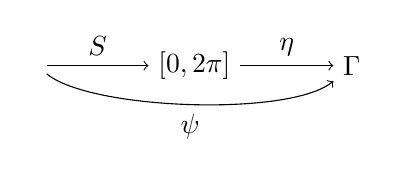
\begin{tikzpicture}[node distance=2cm, auto]
\node (A) {$\del\disk$};
\node(B) [right of=A] {$[0,2\pi]$};
\node (C) [right of=B] {$\Gamma$};
\draw[->](A) to node {$S$}(B);
\draw[->](B) to node {$\eta$}(C);
\draw[->, out = -40, in = -140, looseness = 0.5] (A) to node [below]{$\psi$}(C); % this should be a circular arrow under the diagram
\end{tikzpicture}
$$ 
We improve the approximation by moving the points along their tangents towards the boundary curve, i.e. by finding a correction function $U_k:\del\disk\to[0,2\pi]$ such that
\begin{equation}\label{eq:h_k+1}
    \eta(S_k(\zeta))+U_k(\zeta)\dot\eta(S_k(\zeta)) = \psi_{k+1}(\zeta)
\end{equation}
where $\psi_{k+1}$ is an analytic approximation for $\psi$ on $\overline\Omega$. Note that $\psi_{k+1}$ does not generally take values on $\Gamma$. 
The above equation (\ref{eq:h_k+1}) has two unknowns, $U_k$ and $\psi_{k+1}$, which makes it a \red{Riemann-Hilbert Problem}.
By the Riemann Mapping Theorem, it admits a unique solution only if we fix the mapping normalization. We therefore require that a specific boundary point $z_0$ corresponds to the target parameter $s_0$ (where $\eta(s_0) = c_0$). A direct coordinate constraint $\psi_{k+1}(z_0) = c_0$ is geometrically impossible because $\psi_{k+1}(z_0)$ is constrained to the tangent vector, while $c_0$ lies on the curve $\Gamma$. Therefore, the normalization condition is transferred to the parameter space. We force the updated parameter function to satisfy $S_{k+1}(z_0) = s_0$, which directly yields the necessary boundary condition for $U_k$ \cite[Equation 2.4a]{Wegmann1978_newtonverfahren}:
\begin{equation}
    U_k(z_0)=s_0-S_k(z_0).
\end{equation}

To find $U_k$, equation (\ref{eq:h_k+1}) is rewritten into \cite[Equation 3.4]{Wegmann1978_newtonverfahren}:
\begin{equation}
    \text{Re}(\frac{\psi_{k+1}}{i\dot\eta(S_k(\zeta))})= \text{Im}(\frac{\eta(S_k(\zeta))}{\dot\eta(S_k(\zeta))}).
\end{equation}
This eliminates $U_k$ (since it is real-valued) and yields a boundary value problem for $\psi_{k+1}$ which can be solved using the operator $K$ defined in \ref{operatorK_N}. 
This is done via FFT (see \ref{chap:WegmannImplementation}). Subsequently, $U_k$ is recovered by rearranging equation (\ref{eq:h_k+1}).

Finally, we get an approximation for the parametrization $S$ by 
\begin{equation}
    S_{k+1}(\zeta):= S_k(\zeta)+U_k(\zeta)
\end{equation}
which can be understood as "new guess equals last guess plus some correction".






\begin{algorithm}
    \caption{Wegmann's Method}
    \begin{algorithmic}[1]
        \STATE \textbf{Input:} Target boundary $\eta: [0, 2\pi] \to \mathbb{C}$, anchor points $z_0 \in \partial\mathbb{D}, s_0 \in [0, 2\pi]$.
        \STATE \textbf{Initialize:} $S_0(\zeta) = \arg(\zeta)$ (Identity) or guess satisfying $S_0(z_0)=s_0$.
        \WHILE {not converged}
            \STATE \textit{// 1. Evaluate current boundary geometry}
            \STATE $f_k(\zeta) := \eta(S_k(\zeta))$
            \STATE $g_k(\zeta) := \dot\eta(S_k(\zeta))$
            
            \STATE \textit{// 2. Solve Riemann-Hilbert Problem with anchoring}
            \STATE Find analytic function $\psi_{k+1}$ on $\mathbb{D}$ satisfying:
            \begin{equation*}
                \text{Re}\left(\frac{\psi_{k+1}(\zeta)}{i g_k(\zeta)}\right) = \text{Im}\left(\frac{f_k(\zeta)}{g_k(\zeta)}\right) \quad \forall \zeta \in \partial\mathbb{D}
            \end{equation*}
            \STATE subject to the constraint:
            \begin{equation*}
                 \text{Re}\left(\frac{\psi_{k+1}(z_0) - f_k(z_0)}{g_k(z_0)}\right) = s_0 - S_k(z_0)
            \end{equation*}

            \STATE \textit{// 3. Compute correction and update}
            \STATE $U_k(\zeta) := \text{Re}\left( \frac{\psi_{k+1}(\zeta) - f_k(\zeta)}{g_k(\zeta)} \right)$
            \STATE $S_{k+1}(\zeta) := S_k(\zeta) + U_k(\zeta)$
        \ENDWHILE
    \end{algorithmic}
\end{algorithm}

\subsubsection{Implementation} \label{chap:WegmannImplementation}
Since we assume $\psi$ to map from the unit disk $\disk$, the integral equations can be explicitly solved by discretization and trigonometric interpolation \cite[§5]{Wegmann1978_newtonverfahren}:
Take $N=2n$ equidistant points $\zeta_k=e^{i\theta_k}$ on the boundary of the disk, where
$$\theta_k = \theta_0 + \frac{\pi k}{N}, \quad k\in[N-1]$$
and write the integrals in terms of their Fourier transform
\begin{equation}
    F(z)=\frac{1}{2\pi i}\int \frac{\sigma_n(\zeta)}{\zeta - z} d\zeta
\end{equation}
where
$$\sigma_n(\zeta_k)=\displaystyle\sum_{i=-n}^{n} c_i \zeta_k^i.$$ 
This $\sigma_n \mapsto F$ can be computed fast ($\in\bigO(N\log N)$) via FFT.
% Then, given $\eta(s)$, $\dot\eta(s)$ and $\Theta(s):= arg(\dot\eta(s))$ in closed form, and given initial values $S_1(\zeta_k)$ the next iteration is computed as follows:


Note that this is a Newton method and thus only guaranteed to converge locally due to the linearisation of the boundary. Hence why a "good" (close enough) initial guess is vital for numerical stability. In practice, for $\Omega$ far from circular, a homotopy method could probably be adopted, where each solution for a slightly deformed circle is used as initial guess for the next deformation until the target region is reached.
Unlike the AP Method, which uses a fixed projection to find the next iterate, Wegmann's Method leverages the exact geometry of the boundary curve via $\theta$, which yields quadratic convergence since the error decreases much faster \cite[Theorem 4]{Wegmann1978_newtonverfahren}.
%However, given a suitable initial guess, the method achieves a quadratic local convergence rate for smooth boundaries, or superlinear for sufficiently smooth boundaries \cite{Wegmann1989_alternating_projections}, unlike just linear convergence achieved by standard fixed-set alternating projection methods.

\newpage
\subsection{Comparison}
We can directly rule out some of the options due to our project constraints: 
First we note that Schwarz-Christoffel only works on polygons and Theodorsen's method is restricted to star-shaped regions. Since we want to be able to work with more general shapes of $\Omega$, we disregard these two methods.

We refrain from using probabilistic methods due to their inherent randomness and the difficulty of guaranteeing a certain accuracy, but it is worthwile noting that this is a good choice in cases where the boundary is so rough/ irregular that deterministic methods fail.
Since we are given a smooth boundary of the target domain, we can opt for a more accurate method.

The Zipper method is very well implementable and robust (it can handle rough boundaries including fractals), but there is a small caveat to be aware of for the efficient point evaluations. Since the Zipper method essentially constructs $\psi$ as a composition of many maps, the derivative is numerically expensive to compute (chain rule). Also, trying a finite differences approach is slow and potentially numerically unstable, but there is hope in a technique called Forward Automatic Differentiation which is both exact and efficient \cite{wikipedia_autodiff}. 

The Conjugate Function Method contains a very astute idea mathematically, but its implementation is not very interesting beyond $hp$-FEM for which there already are powerful libraries, so there would not be much value in implementing a rudimentary FEM solver given the scope of this thesis. 

Amano's Method of Fundamental Solutions seems good for fast (linear time) point-evaluations of $\psi$ as well as its derivative as it is a sum of simple fractions and all the singularities (charge points) are placed strictly outside the region. However, we cannot directly use our Fourier parametrization nor our mesh in this method, so it will probably not be the best choice for our specific problem. Note also that the accuracy and convergence of this method depend on the right choice of charge points.

Lastly, Wegmann's Method and the Method of Alternating Projections both use the boundary parametrization in its Fourier series form.
In both cases, the output is an interpolating polynomial, allowing for efficient point evaluations of $\psi$ and $D\psi$ \cite{Wegmann1984_convergence_iterative_method}.
The AP Method is one of the simplest and most robust methods for conformal mapping. However, it is not very accurate for reasonably sized grids, and converges only linearly \cite[Chapter 4.2]{Wegmann2005_num_methods_confmapping}.
In contrast, Newton's Method converges quadratically for analytic boundaries (as is known for Newton methods) and superlinear ($\in\bigO(N^{1+\mu})$) for $\eta\in C^{2+\mu}$ but depends on a "good enough" initial guess for the boundary correspondence function (\ref{eq:boundaryCorrespondence}) \cite[§ 4]{Wegmann1978_newtonverfahren}, \cite[page 292]{Wegmann1989_alternating_projections}, \cite{Wegmann1984_convergence_iterative_method}.


%Wegmann compared the accuracies of the AP, OAP, Theodorsen and Wegmann methods for the mapping from the disk to an inverted ellipse and found that OAP is most efficient for low accuracy and Newton methods are best for slower high accuracy calculations \cite[p. 415]{Wegmann2005_num_methods_confmapping}.
%Note the computational costs of these last two methods are mainly determined by the FFTs and this parameter is dependent on the number of grid points.

Hence, both Zipper, AP and Wegmann's methods seem suitable for our problem, but Wegmann's Method is most accurate with fastest convergence while seemingly the most interesting to implement.
The Zipper method is also very appealing due to its robustness, but since we are given a smooth boundary and want high accuracy, we can afford to use a method that is less robust but more accurate.
We will therefore opt for implementing Wegmann's Method.
\bigskip

\begin{sidewaystable}[htbp]
    \centering
    \small
    \caption{Comparison of Numerical Conformal Mapping Methods}
    \label{tab:method_comparison}
    \renewcommand{\arraystretch}{1.5} % Good vertical spacing
    
    % The sum of the hsize values below MUST equal 7 (the number of columns)
    \begin{tabularx}{\textwidth}{@{} 
        >{\hsize=0.7\hsize\raggedright\arraybackslash}X  % 1. Method (Narrow)
        >{\hsize=0.7\hsize\raggedright\arraybackslash}X  % 2. Shape (Very Narrow)
        >{\hsize=0.6\hsize\raggedright\arraybackslash}X  % 3. Runtime (Narrow)
        >{\hsize=0.8\hsize\raggedright\arraybackslash}X  % 4. Input (Medium)
        >{\hsize=0.9\hsize\raggedright\arraybackslash}X  % 5. Output (Wide)
        >{\hsize=1.65\hsize\raggedright\arraybackslash}X % 6. Advantages (Very Wide)
        >{\hsize=1.65\hsize\raggedright\arraybackslash}X % 7. Disadvantages (Very Wide)
    @{}}
        \toprule
        \textbf{Method} & \textbf{$\Omega$ Shape} & \textbf{Runtime} & \textbf{Input} & \textbf{Output} & \textbf{Advantages} & \textbf{Disadvantages} \\
        \midrule
        
        \textbf{Schwarz-Christoffel} & 
        Polygon & 
        $\bigO(N^3)$ (parameter problem) & 
        Polygon vertices $z_k$ and angles $\theta_k$& 
        Integral parameters: prevertices $v_k$, $C$ & 
        Exact angle preservation at corner singularities; Handles unbounded \& periodic domains. & 
        Restricted to polygons; Crowding (resolution loss); Slow \\
        \addlinespace
        
        \textbf{Theodorsen} & 
        Star-shaped & 
        $\bigO(N \log N)$ & 
        Radial function $\rho(\theta)$ & 
        Boundary correspondence $\theta(\phi)$ & 
        Fast fixed-point iteration; Efficient FFT implementation. & 
        Restricted to star-shaped regions; Fails/Inaccurate for non-smooth boundaries or shapes far from $\disk$. \\
        \addlinespace
        
        \textbf{Zipper (Geodesic)} & 
        General Jordan incl. Fractals & 
        Fast, Dep. only on $N$ but not on shape & 
        Boundary points $\{z_i\}_{i\in[N]}$ & 
        Composition of elementary maps & 
        Robust (handles fractals); Finds inverse simultaneously. & 
        Expensive derivative computation (chain rule); Only approximates $\Gamma$. \\
        \addlinespace
        
        \textbf{Alternating Projections} & 
        Smooth & 
        $\bigO(N \log N)$ per iter.: FFT & 
        Fourier Series of $\eta$ & 
        Interpolating Polynomial & 
        Robust and simple to implement; Efficient point evaluation. & 
        Linear (slow) convergence for fine meshes; Low accuracy for reasonable grids. \\
        \addlinespace
        
        \textbf{Wegmann's Method} & 
        Smooth & 
        $\bigO(N \log N)$ per iter.: FFT & 
        $\eta$ and tangent angles & 
        Analytic function (Trig. poly) & 
        Quadratic (fast) convergence for fine meshes; High accuracy (FFT); Efficient point evaluation. & 
        Requires good initial guess; Complex implementation. \\
        \addlinespace
        
        \textbf{Amano's Method} & 
        Analytic & 
        $\bigO(N^3)$ & 
        Collocation points $z_i$ & 
        Lin. comb. of log potentials & 
        Fast linear point/derivative evaluation; Exponential accuracy; Simple implementation. & 
        Cannot use Fourier param. or mesh; Sensitive to charge point placement. \\
        \addlinespace
        
        \textbf{Probabilistic Method} & 
        General, incl. Rough/ Fractals & 
        Polynomial & 
        Oracle / Boundary (pixel list) & 
        Random Walk approx. & 
        Works on rough boundaries where deterministic methods fail. & 
        Slow convergence; Inherent randomness; Difficult to guarantee accuracy. \\
        
        \bottomrule
    \end{tabularx}
\end{sidewaystable}